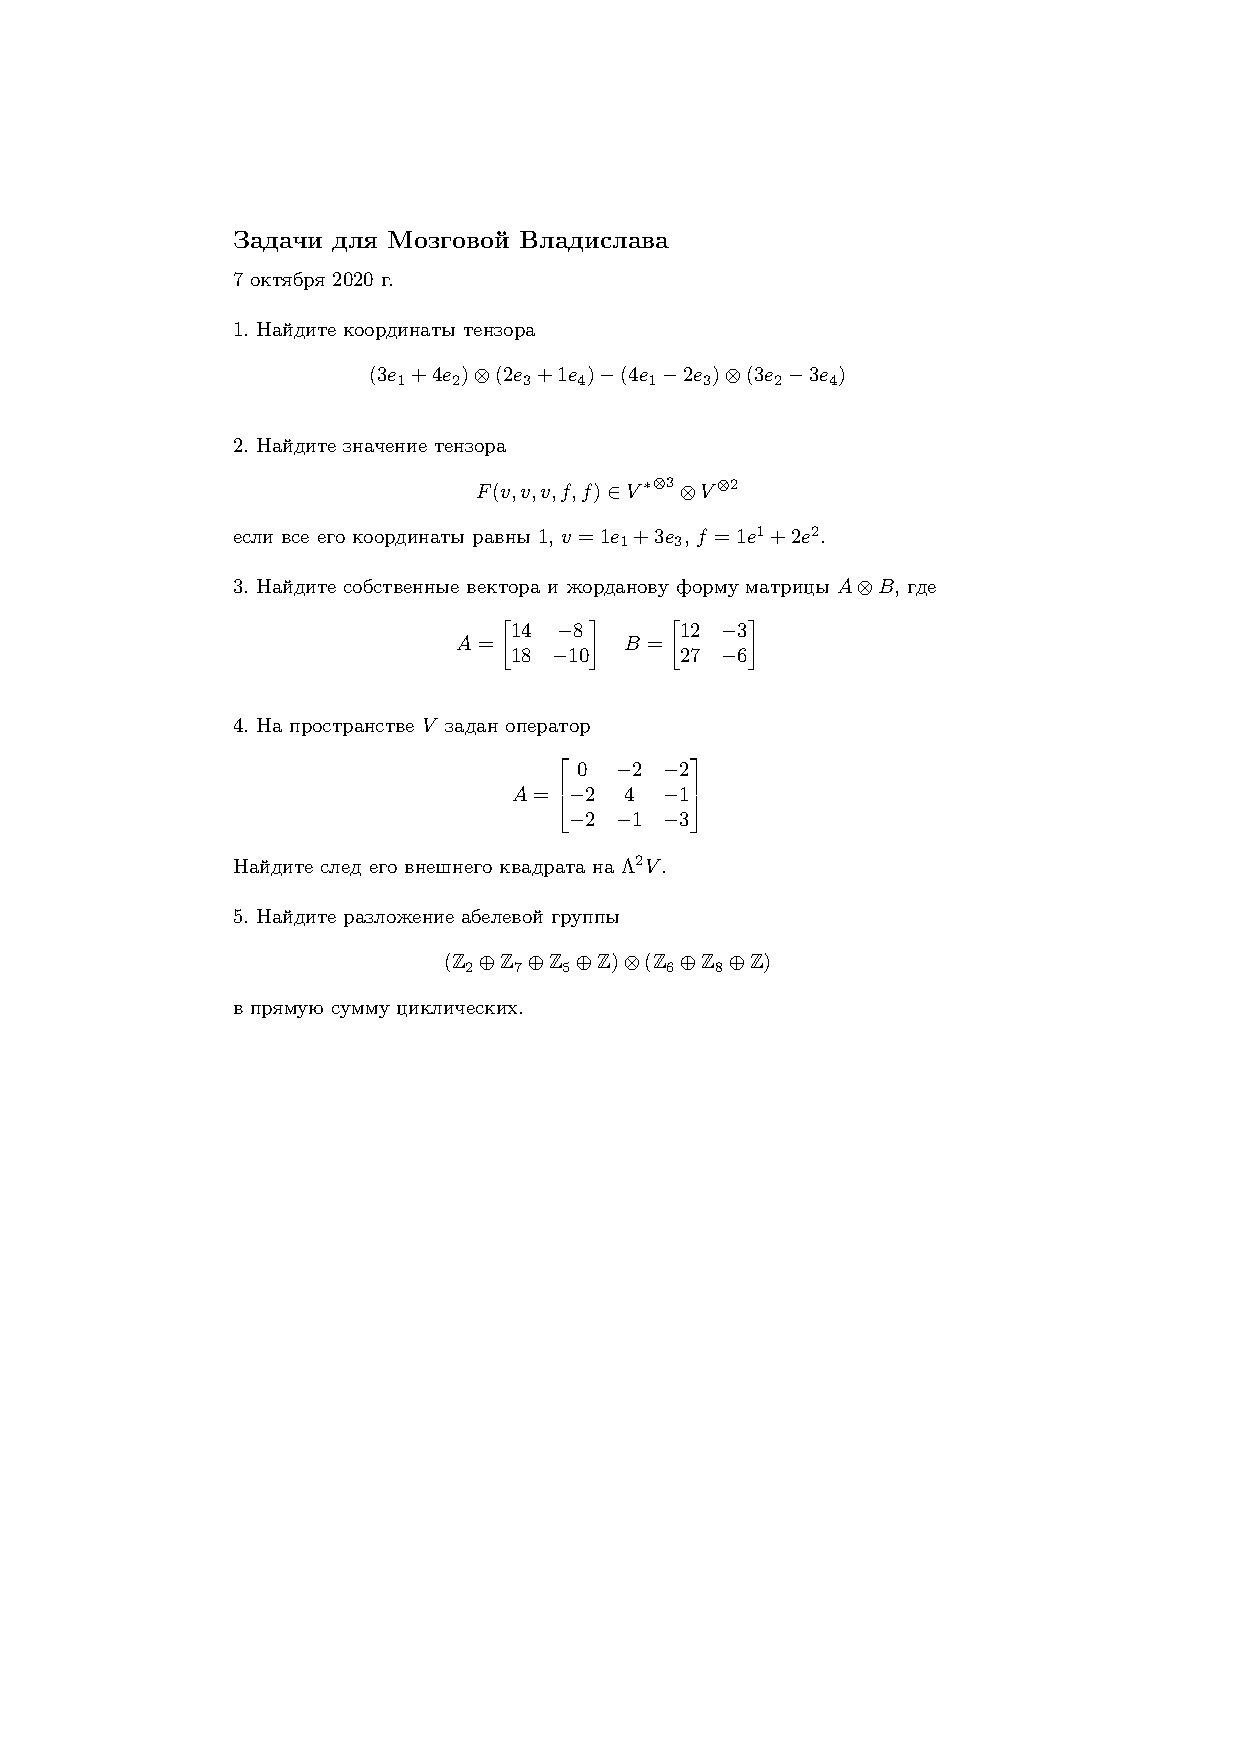
\includepdf[scale=0.95,pages=1,pagecommand=\section*{Условия}]{Tasks/problem1}
\newpage
\section*{Решения}
\subsection*{Задача 1}
\begin{gather*}
	(3e_1 + 4e_2) \otimes (2e_3 + 1e_4) - (4e_1 - 2e_3) \otimes (3e_2 - 3e_4) = \\
	(6 e_1 \otimes e_3 + 3 e_1 \otimes e_4 + 8 e_2 \otimes e_3 + 4 e_2 \otimes e_4) - (12 e_1 \otimes e_2 - 12e_1 \otimes e_4 - 6e_3 \otimes e_2 + 6e_3 \otimes e_4) =\\
	-12e_1 \otimes e_2 + 6e_1 \otimes e_3 + 15e_1 \otimes e_4 + 8e_2 \otimes e_3 + 4e_2 \otimes e_4 + 6e_3 \otimes e_2 - 6e_3 \otimes e_4
\end{gather*}
Тензорное умножение пространств с базисами $\{e_1, e_2, e_3, e_4\}$ это сложение его элементов, п следовательно базис пространства, элементы которого мы складываем, это векторы $e_i \otimes e_j$, то есть
\begin{gather*}
\begin{matrix}
	e_1 \otimes e_1 & e_1 \otimes e_2 & e_1 \otimes e_3 & e_1 \otimes e_4\\
	e_2 \otimes e_1 & e_2 \otimes e_2 & e_2 \otimes e_3 & e_2 \otimes e_4\\
	e_3 \otimes e_1 & e_3 \otimes e_2 & e_3 \otimes e_3 & e_3 \otimes e_4\\
	e_4 \otimes e_1 & e_4 \otimes e_2 & e_4 \otimes e_3 & e_4 \otimes e_4
\end{matrix}
\end{gather*}
тогда координаты тензора это:
\begin{gather*}
\begin{pmatrix}
	0 & -12 & 6 & 15\\
	0 & 0 & 8 & 4\\
	0 & 6 & 0 & -6\\
	0 & 0 & 0 & 0
\end{pmatrix}
\end{gather*}

\subsection*{Задача 2}
$F \in V^{* \otimes 3} \otimes V^{\otimes 2}$ 
\begin{gather*}
	v = 1e_1 + 3e_3\\
	f = 1e^1 + 2e^2\\
	F(e_{i_1}, e_{i_2}, e_{i_3}, e^{i_4}, e^{i_5}) = a_{i_1 i_2 i_3}^{i_4 i_5}\ \text{по условию все координаты 1}\\
	(e^{j_1} \otimes e^{j_2} \otimes e^{j_3} \otimes e_{j_4} \otimes e_{j_5})(e_{i_1}, e_{i_2}, e_{i_3}, e^{i_4}, e^{i_5}) = e^{j_1}(e_{i_1}) e^{j_2}(e_{i_2}) e^{j_3}(e_{i_3}) e^{i_4}(e_{j_4}) e^{i_5}(e_{j_5}) =\\
	=
	\begin{cases}
		1\quad i_1 = j_1,\ i_2 = j_2,\ i_3 = j_3,\ i_4 = j_4,\ i_5 = j_5\\
		0\quad \text{во всех остальных случаях}
	\end{cases}\\
	F(v,v,v,f,f) = (1+3)(1+3)(1+3)(1+2)(1+2) = 576
\end{gather*}



\subsection*{Задача 3}
\begin{gather*}
	A = 
	\begin{bmatrix}
		14 & -8 \\ 18 & -10
	\end{bmatrix}
	\qquad
	B = 
	\begin{bmatrix}
		12 & -3 \\ 27 & -6
	\end{bmatrix}
\end{gather*}
Найдем собственные числа и вектора этих матриц
\begin{gather*}
	\begin{bmatrix}
		14 - \lambda_A & -8\\
		18 & -10-\lambda_A
	\end{bmatrix}
	= \lambda_A^2 - 4\lambda_A + 4 = (\lambda_A - 2)^2\\
	A - \lambda_A E = 
	\begin{bmatrix}
		12 & -8\\
		18 & -12
	\end{bmatrix}
	= 
	\begin{bmatrix}
		3 & -2\\
		0 & 0
	\end{bmatrix}\\
	x_1 = \frac{2}{3} x_2
\end{gather*}
и
\begin{gather*}
	\begin{bmatrix}
		12 - \lambda_B & -3\\
		27 & -6 - \lambda_B
	\end{bmatrix}
	= \lambda_B^2 - 6\lambda_B + 9 = (\lambda_B - 3)^2\\
	B - \lambda_B E = 
	\begin{bmatrix}
		9 & -3\\
		27 & -9
	\end{bmatrix}
	=
	\begin{bmatrix}
		3 & -1\\
		0 & 0
	\end{bmatrix}\\
	x_1 = -\frac{1}{3} x_2
\end{gather*}

\vskip 0.3in
Теперь найдем Жорданову форму
\begin{gather*}
	A = 
	\begin{bmatrix}
	14 & -8 \\ 18 & -10
	\end{bmatrix}\\
	\lambda = 2
\end{gather*}
\begin{enumerate}
\item 
	$\left(\begin{bmatrix}
	14 & -8\\ 18 & -10
	\end{bmatrix} - 2E\right)^2$ 
	\begin{gather*}
		\left(\begin{bmatrix}
			14 & -8\\ 18 & -10
		\end{bmatrix} - 2E\right)^2
		\cdot
		\begin{pmatrix}
			1 \\ 0
		\end{pmatrix}
		=
		\begin{pmatrix}
			12 \\ 18
		\end{pmatrix}
	\end{gather*}
	\vskip 0.1in
	\begin{gather*}
		\left(\begin{bmatrix}
			14 & -8\\ 18 & -10
		\end{bmatrix} - 2E\right)^2
		\cdot
		\begin{pmatrix}
			0 \\ 1
		\end{pmatrix}
		=
		\begin{pmatrix}
			-8 \\ -12
		\end{pmatrix}
	\end{gather*}

\item 
	$\left(\begin{bmatrix}
	14 & -8\\ 18 & -10
	\end{bmatrix} - 2E\right)^1$
	\begin{gather*}
		\left(\begin{bmatrix}
		14 & -8\\ 18 & -10
		\end{bmatrix} - 2E\right)^1
		\cdot
		\begin{pmatrix}
			\frac{2}{3} \\ 1
		\end{pmatrix}
	\end{gather*}
\end{enumerate}
Откуда 
\begin{gather*}
	M = 
	\begin{bmatrix}
		12 & 1 \\ 18 & 0
	\end{bmatrix}\\
	J_A = 
	\begin{bmatrix}
		2 & 1 \\ 0 & 2
	\end{bmatrix}
\end{gather*}


\begin{gather*}
	B = 
	\begin{bmatrix}
		12 & -3 \\ 27 & -6
	\end{bmatrix}\\
	\lambda = 3
\end{gather*}
\begin{enumerate}
	\item 
	$\left(\begin{bmatrix}
		12 & -3\\ 27 & -6
	\end{bmatrix} - 3E\right)^2$ 
	\begin{gather*}
	\left(\begin{bmatrix}
		12 & -3\\ 27 & -6
	\end{bmatrix} - 3E\right)^2
	\cdot
	\begin{pmatrix}
		1 \\ 0
	\end{pmatrix}
	=
	\begin{pmatrix}
		9 \\ 27
	\end{pmatrix}
	\end{gather*}
	\vskip 0.1in
	\begin{gather*}
	\left(\begin{bmatrix}
		12 & -3\\ 27 & -6
	\end{bmatrix} - 2E\right)^2
	\cdot
	\begin{pmatrix}
		0 \\ 1
	\end{pmatrix}
	=
	\begin{pmatrix}
		-3 \\ -9
	\end{pmatrix}
	\end{gather*}
	
	\item 
	$\left(\begin{bmatrix}
		12 & -3\\ 27 & -6
	\end{bmatrix} - 3E\right)^1$ 
	\begin{gather*}
	\left(\begin{bmatrix}
		12 & -3\\ 27 & -6
	\end{bmatrix} - 3E\right)^1
	\cdot
	\begin{pmatrix}
		\frac{1}{3} \\ 1
	\end{pmatrix}
	\ne 0
	\end{gather*}
\end{enumerate}
Откуда 
\begin{gather*}
	M = 
	\begin{bmatrix}
		9 & 1 \\ 27 & 0
	\end{bmatrix}\\
	J_B = 
	\begin{bmatrix}
		3 & 1 \\ 0 & 3
	\end{bmatrix}
\end{gather*}
\vskip 0.2in
Тогда собственные значения и вектора $A \otimes B$ имеют вид:
\begin{gather*}
	\lambda = \lambda_A \cdot \lambda_B = 2 \cdot 3 = 6\\
	\begin{pmatrix}
	-\frac{1}{3}a + \frac{4}{9}b\\
	-a + b\\
	a\\
	b
	\end{pmatrix}\\
\end{gather*}
Откуда
\begin{gather*}
	a = 1, b = 0\qquad 
	\begin{pmatrix}
		-\frac{1}{3}\\ -1\\ 1\\ 0
	\end{pmatrix}
	\\
	a = 0, b = 1\qquad
	\begin{pmatrix}
		\frac{4}{9}\\ 1\\ 0\\ 1
	\end{pmatrix}
\end{gather*}
и жорданова форма имеет вид
\begin{gather*}
	J_A \otimes J_B = 
	\begin{bmatrix}
		2 & 1 \\ 0 & 2
	\end{bmatrix}
	\otimes
	\begin{bmatrix}
		3 & 1 \\ 0 & 3
	\end{bmatrix}
	=
	\begin{bmatrix}
		6 & 3 & 3 & 1\\
		0 & 6 & 0 & 1\\
		0 & 0 & 6 & 3\\
		0 & 0 & 0 & 6
	\end{bmatrix}
	=
	\begin{bmatrix}
		6 & 1 & 0 & 0\\
		0 & 6 & 1 & 0\\
		0 & 0 & 6 & 0\\
		0 & 0 & 0 & 6
	\end{bmatrix}
\end{gather*}


\subsection*{Задача 4}
Пусть $e_1,e_2,e_3$ -- базисные векторы
\begin{gather*}
	e_1 \land e_2 = e_1 \otimes e_2 - e_2 \otimes e_1\\
	e_2 \land e_3 = e_2 \otimes e_3 - e_3 \otimes e_2\\
	e_3 \land e_1 = e_3 \otimes e_1 - e_1 \otimes e_3
\end{gather*}
Пусть 
\begin{gather*}
B = 
\begin{pmatrix}
	a & b & c\\
	d & f & g\\
	x & y & z
\end{pmatrix}
\end{gather*}
Тогда
\begin{gather*}
	e_1 \otimes e_2 \rightarrow (ae_1 + de_2 + xe_3) \otimes (be_1 + fe_2 + ye_3)\\
	e_1 \land e_2 = (ae_1 + de_2 + xe_3) \otimes (be_1 + fe_2 + ye_3) - (be_1 + fe_2 + ye_3) \otimes (ae_1 + de_2 + xe_3) =\\
	(af - bd)(e_1 \otimes e_2 - e_2 \otimes e_1) + (ay - bx)(e_1 \otimes e_3 - e_3 \otimes e_1) + (dy - fx)(e_2 \otimes e_3 - e_3 \otimes e_2) =\\
	B_{33} e_1 \land e_2 + (ay - bx)e_1 \land e_3 + (dy - fx)e_2 \land e_3
\end{gather*}
Аналогично распишем $e_2 \land e_3$ и $e_1 \land e_3$\\
\begin{comment}
\begin{gather*}
e_2 \land e_3 = (bg - cf)(e_1 \otimes e_2 - e_2 \otimes e_1) + (bz - cy)(e_1 \otimes e_3 - e_3 \otimes e_1) + (fz - gy)(e_2 \otimes e_3 - e_3 \otimes e_2)
\end{gather*}
И
\begin{gather*}
e_1 \land e_3 = (az - cx)(e_1 \otimes e_2 - e_2 \otimes e_1) + (bz - cy)(e_1 \otimes e_3 - e_3 \otimes e_1) + (fz - gy)(e_2 \otimes e_3 - e_3 \otimes e_2)
\end{gather*}
\end{comment}
Тогда $\land^2V$ Представим в виде матрицы
\begin{gather*}
B'= 
\begin{pmatrix}
	B_{11} & \ldots & \ldots\\
	\ldots & B_{22} & \ldots\\
	\ldots & \ldots & B_{33}
\end{pmatrix}\\
\operatorname{tr}B' = \sum\limits_{i = 1}^{3} B_{ii}
\end{gather*}
Тогда для $A$
\begin{gather*}
A = 
\begin{pmatrix}
	0 & -2 & -2\\
	-2 & 4 & -1\\
	-2 & -1 & -3
\end{pmatrix}\\
A' =
\begin{pmatrix}
	-13 & 4 & 10\\
	4 & -4 & -4\\
	10 & -4 & -4
\end{pmatrix}\\
\operatorname{tr}A'= \sum\limits_{i = 1}^{3} = -13 + (-4) + (-4) = -21
\end{gather*}



\subsection*{Задача 5}
Заметим, что $\mathbb{Z}\backslash_k \otimes \mathbb{Z}\backslash_l = \langle 0 \rangle\quad (k,l) = 0$, так как $la \otimes b = l(a \otimes b) = a \otimes lb = 0$\\
И $\mathbb{Z}\backslash_k \otimes \mathbb{Z} = \langle 0 \rangle$, так как $a \otimes kb = ka \otimes b = 0$
\vskip 0.2in
Также заметим что $(A \otimes B) \otimes C = A \otimes C \oplus B \otimes C$, откуда следует что\\
\begin{gather*}
	(\mathbb{Z}_2 \oplus \mathbb{Z}_7 \oplus \mathbb{Z}_5 \oplus \mathbb{Z}) \otimes (\mathbb{Z}_6 \oplus \mathbb{Z}_8 \oplus \mathbb{Z}) = \mathbb{Z}_2 \otimes \mathbb{Z}_6 \oplus \mathbb{Z}_2 \otimes \mathbb{Z}_8
\end{gather*}
Тогда осталось заметить что $\mathbb{Z}\backslash_k \otimes \mathbb{Z}\backslash_l = \mathbb{Z}\backslash_{(k,l)}$, откуда
\begin{gather*}
	\mathbb{Z}_2 \otimes \mathbb{Z}_6 = \mathbb{Z}_2\\
	\mathbb{Z}_2 \otimes \mathbb{Z}_8 = \mathbb{Z}_2
\end{gather*}
Следовательно разложение имеет вид $\mathbb{Z}_2 \oplus \mathbb{Z}_2$